\documentclass[11pt]{article}

\usepackage[a4paper,margin=25mm]{geometry}
\usepackage{amsmath,amssymb,amsthm,mathtools}
\usepackage{booktabs}
\usepackage{enumitem}
\usepackage{graphicx}
\usepackage[hidelinks]{hyperref}
\usepackage{xcolor}

\newcommand{\Eset}{\mathcal{E}}
\newcommand{\SLZ}{\mathrm{SL}(2,\mathbb{Z})}
\newcommand{\GLZ}{\mathrm{GL}(2,\mathbb{Z})}
\newcommand{\trans}{\mathsf{T}}

\title{Unit-Step versus Batched Plastic Reduction\\
\large Exact Non-Equivalence and Lattice Equivalence}
\author{Technical note}
\date{14 July 2026}

\begin{document}
\maketitle

\begin{abstract}
The unit-step and nearest-integer-shear versions of the two-dimensional
plastic-reduction algorithm are \emph{not} identical algorithms: even in exact
rational arithmetic, they can terminate at different matrices in the elastic
domain.  The difference is therefore not caused by floating-point error.
What is true is an exact lattice-equivalence statement.  Every output of either
algorithm is related to the input, and hence to the other output, by an integer
unimodular congruence.  After a consistent canonicalization to one fundamental
wedge, generic interior outputs agree.  This note proves these statements and
gives a counterexample whose initial point has Poincare radius approximately
$0.636$.
\end{abstract}

\section{Setting and the two algorithms}

Write a symmetric positive-definite metric as
\[
 C=\begin{pmatrix}a&c\\c&b\end{pmatrix},\qquad
 a>0,\quad b>0,\quad ab-c^2>0,
\]
and define the elastic domain
\[
 \Eset
 =\left\{C\succ0:\ |c|\leq\frac12\min(a,b)\right\}.
\]
The upper and lower integer shears are
\[
 U_m=\begin{pmatrix}1&m\\0&1\end{pmatrix},
 \qquad
 V_m=\begin{pmatrix}1&0\\m&1\end{pmatrix},
 \qquad m\in\mathbb{Z}.
\]
They act by congruence, $C\mapsto W^\trans C W$.  Explicitly,
\begin{align}
 U_m^\trans C U_m
 &=
 \begin{pmatrix}
 a & c+ma\\
 c+ma & b+2mc+m^2a
 \end{pmatrix}, \label{eq:U-update}\\
 V_m^\trans C V_m
 &=
 \begin{pmatrix}
 a+2mc+m^2b & c+mb\\
 c+mb & b
 \end{pmatrix}. \label{eq:V-update}
\end{align}

Outside $\Eset$, the current unit-step implementation chooses
\[
 \begin{cases}
 U_{-\operatorname{sgn}(c)},&a\leq b,\\
 V_{-\operatorname{sgn}(c)},&b<a,
 \end{cases}
\]
then tests the branch and stopping conditions again.  The batched candidate
instead uses the nearest integer
\[
 m=
 \begin{cases}
 \operatorname{nint}(-c/a),&a\leq b,\\
 \operatorname{nint}(-c/b),&b<a.
 \end{cases}
\]
The sampled test used round-half-away-from-zero, but the counterexample below
does not lie on a half-integer tie.

\section{What can and cannot be batched}

For $s\in\{-1,1\}$ and $k\in\mathbb{N}$,
\[
 U_s^k=U_{ks},\qquad V_s^k=V_{ks}.
\]
Consequently,
\[
 (U_s^k)^\trans C U_s^k=U_{ks}^\trans C U_{ks},
\]
and similarly for $V$.  Thus a batched shear is algebraically identical to a
fixed run of unit shears in the \emph{same direction}.

This identity does not prove equivalence of the adaptive algorithms.  The
unit-step method retests both $a\leq b$ and membership in $\Eset$ after every
step.  During the putative run it may change from $U$ to $V$, or stop.  A
nearest-integer shear commits to the entire translation before making either
decision.  Therefore it can cross a decision boundary that the unit algorithm
would have detected.

\section{Exact counterexample away from the disk boundary}

Consider the rational metric
\[
 C_0=
 \begin{pmatrix}
 1&-151/100\\
 -151/100&3
 \end{pmatrix},
 \qquad
 \det C_0=\frac{7199}{10000}>0.
\]
The initial nearest-integer quotient is $151/100$, so the batched choice is
unambiguously $m=2$.

\subsection*{Unit-step path}

The unit method first applies $U_1$:
\[
 C_1^{(u)}=U_1^\trans C_0U_1
 =
 \begin{pmatrix}
 1&-51/100\\
 -51/100&49/50
 \end{pmatrix}.
\]
Now $b<a$ and $51/100>(49/50)/2=49/100$, so it does not stop; it
applies $V_1$ and obtains
\[
 C_u=V_1^\trans C_1^{(u)}V_1
 =
 \begin{pmatrix}
 24/25&47/100\\
 47/100&49/50
 \end{pmatrix}.
\]
This endpoint lies strictly inside $\Eset$ because
$47/100<\tfrac12(24/25)=48/100$.

\subsection*{Batched path}

The batched method first applies $U_2$:
\[
 C_1^{(b)}=U_2^\trans C_0U_2
 =
 \begin{pmatrix}
 1&49/100\\
 49/100&24/25
 \end{pmatrix}.
\]
It then applies $V_{-1}$ and obtains
\[
 C_b=V_{-1}^\trans C_1^{(b)}V_{-1}
 =
 \begin{pmatrix}
 49/50&-47/100\\
 -47/100&24/25
 \end{pmatrix}.
\]
This endpoint is also strictly inside $\Eset$.  In particular,
\[
 C_u\neq C_b
\]
in exact rational arithmetic.  The difference is order one and cannot be
attributed to floating-point roundoff.

The Poincare coordinates used by the plotting code are
\[
 x_p=\frac{a-b}{a+b+2\sqrt{\det C}},
 \qquad
 y_p=\frac{2c}{a+b+2\sqrt{\det C}}.
\]
For $C_0$ this gives
\[
 (x_p,y_p)
 =
 \left(
 -\frac{100}{200+\sqrt{7199}},
 -\frac{151}{200+\sqrt{7199}}
 \right)
 \approx(-0.3511,-0.5301),
\]
with radius $r_p\approx0.6358$.  Hence the phenomenon occurs well inside the
disk, not only near its numerically ill-conditioned boundary.

\begin{figure}[htbp]
 \centering
 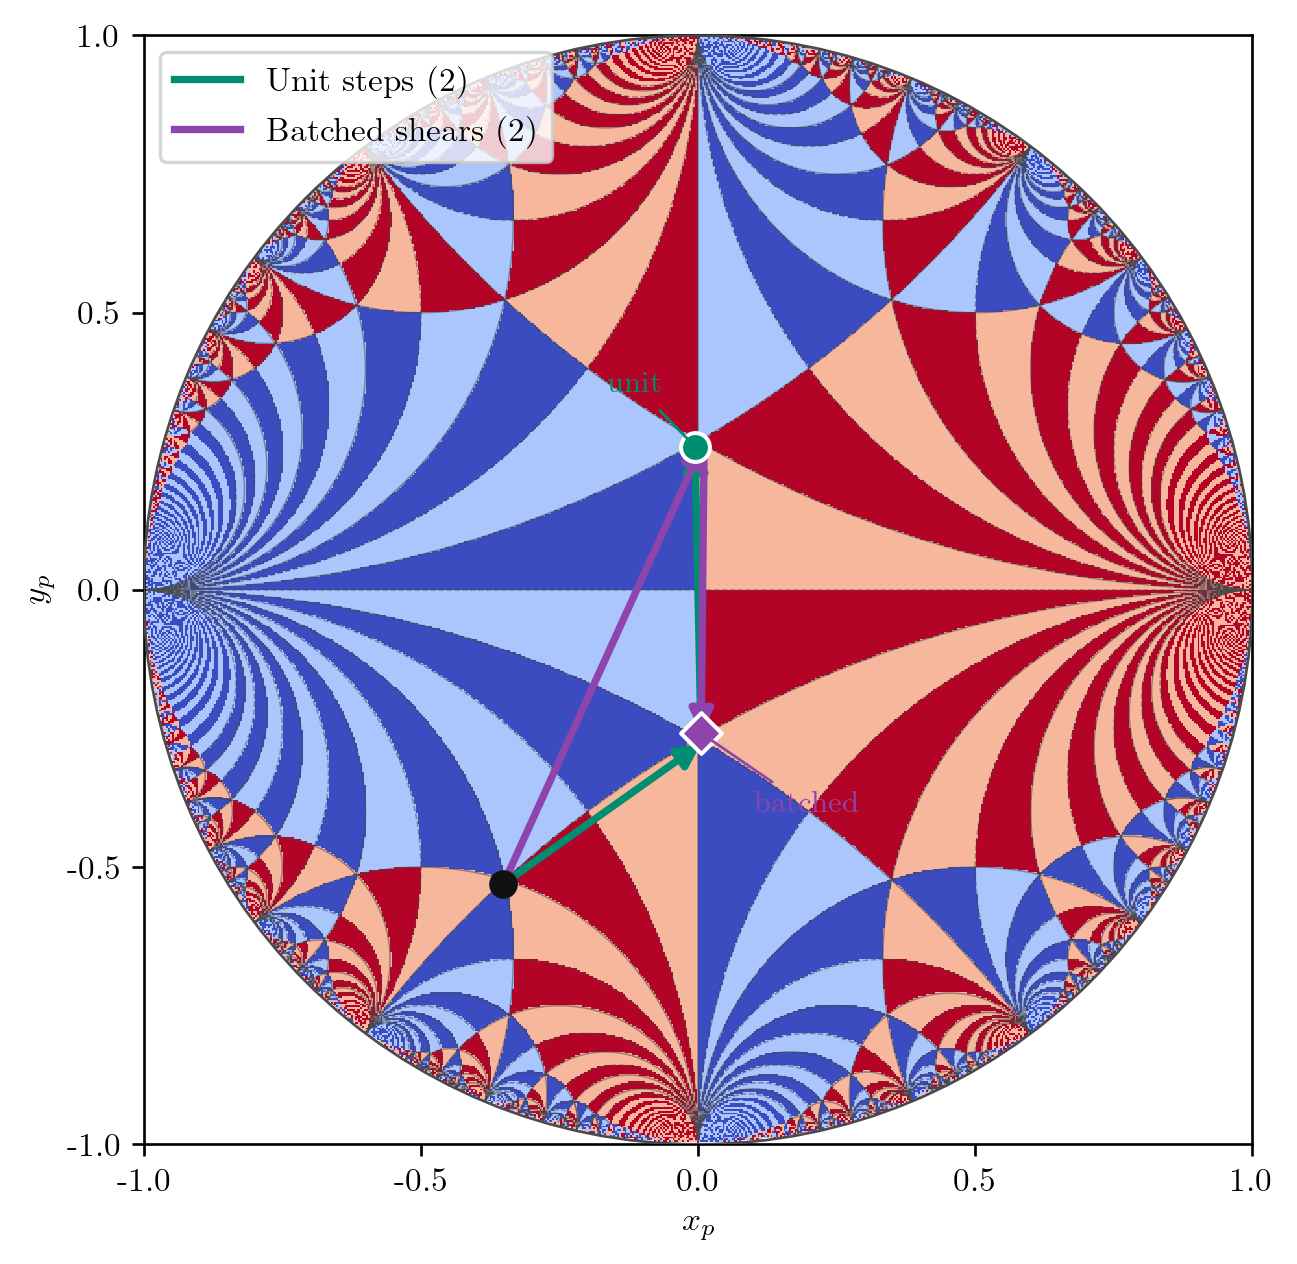
\includegraphics[width=0.68\textwidth]{../../Plots/plastic_reduction_near_center_counterexample.png}
 \caption{The exact rational counterexample.  The green unit-step path and the
 purple batched path start at the same interior point and terminate at
 different representatives of the elastic domain.}
 \label{fig:counterexample}
\end{figure}

\section{The equivalence that is exact}

\subsection{Unimodular-orbit equivalence}

\paragraph{Proposition.}
Assume both algorithms terminate.  Let $M_u,M_b\in\SLZ$ be their accumulated
right-acting transformations, so that
\[
 C_u=M_u^\trans C_0M_u,\qquad
 C_b=M_b^\trans C_0M_b.
\]
Then $C_u$ and $C_b$ are exactly congruent under $\SLZ$.

\paragraph{Proof.}
Set $Q=M_u^{-1}M_b\in\SLZ$.  Then
\[
 Q^\trans C_uQ
 =Q^\trans M_u^\trans C_0M_uQ
 =(M_uQ)^\trans C_0(M_uQ)
 =M_b^\trans C_0M_b
 =C_b.
 \qed
\]

For the counterexample,
\[
 M_u=U_1V_1=
 \begin{pmatrix}2&1\\1&1\end{pmatrix},
 \qquad
 M_b=U_2V_{-1}=
 \begin{pmatrix}-1&2\\-1&1\end{pmatrix},
\]
and
\[
 Q=M_u^{-1}M_b=
 \begin{pmatrix}0&1\\-1&0\end{pmatrix}.
\]
Indeed,
\[
 C_b=Q^\trans C_uQ.
\]
Thus the endpoints represent the same lattice state but are not the same
matrix representative.

\subsection{Energy and canonical representatives}

If the energy satisfies the material symmetry
\[
 \Phi(Q^\trans CQ)=\Phi(C)\qquad(Q\in\GLZ),
\]
then the two endpoints have exactly the same energy in exact arithmetic.
This is the physically relevant equivalence for a $\GLZ$-invariant model.
Tensor components, path histories, and the accumulated transformation matrices
need not be identical.

To demand a unique matrix output, one must additionally canonicalize the
elastic endpoint to a chosen half-open fundamental wedge, for example
\[
 \mathcal{F}
 =\left\{C\succ0:\ a\leq b,\quad 0\leq c\leq a/2\right\},
\]
with explicit boundary tie rules.  The map
\[
 \tau(C)=\frac{c+i\sqrt{\det C}}{a}
\]
sends $\mathcal{F}$ to half of the standard modular fundamental domain:
$|\tau|\geq1$ and $0\leq\operatorname{Re}\tau\leq1/2$.
The standard interior uniqueness of the modular fundamental domain then implies
that two lattice-equivalent, strictly reduced endpoints have the same
canonical representative.  Boundary points still require a prescribed
half-open convention.

For the counterexample, sign normalization followed by diagonal ordering maps
$C_b$ exactly to $C_u$.  This explains why the two paths can be physically
equivalent even though the raw matrices disagree.

\section{Numerical evidence and conclusion}

On the $300\times300$ Cartesian grid in the Poincare disk, there were $70\,168$
strictly interior samples.  Comparing the raw endpoints,
$62\,580$ agreed within relative and absolute tolerances of $10^{-12}$, while
$7\,588$ did not.  A subsequent symmetry classification mapped all sampled
endpoint pairs to one another by diagonal exchange and/or off-diagonal sign
change to numerical precision.  These observations agree with the exact
analysis: the raw algorithms are not exactly equivalent; their outputs remain
in the same integer-unimodular orbit; a canonicalization step is needed if
downstream code requires the same matrix representative; and large-radius
inputs can amplify floating-point error, but roundoff is not the cause of the
representative change.

Therefore a nearest-integer batched implementation is safe only when the
application compares states modulo lattice symmetry, or when it canonicalizes
the final result.  It is not a drop-in replacement if the exact raw endpoint,
the path, or the accumulated transformation is part of the required output.

\end{document}
